\section{Аналитическая часть}

В этом разделе производится анализ предметной области, рассматриваются существующие решения задачи выдачи сертификатов, подтверждающих окончание учебного заведения. Также в данном разделе выбираются средства разработки блокчейн-сети и алгоритм консенсунса сети, рассмотрены их положительные и отрицательные стороны. Также в этом разделе производится формализация постановки задачи и представлена диаграмма IDEF0.

\subsection{Аналоги сертификатов, подтверждающих окончание учебного заведения}

Рассмотрим существующие реализации выдачи сертификатов, подтверждающих окончание учебного заведения:
\begin{itemize}[leftmargin=1.6\parindent]
	\item[---] сертификаты, выдаваемые образовательными онлайн-платформами, такими как Coursera \cite{coursera};
	\item[---] документы об окончания вуза РФ.
\end{itemize}

Сертификаты, выдаваемые образовательными онлайн-платформами, представляют из себя файл, в котором отражена информация о выпускнике и курсе, который он закончил. Такой документ подвержен фальсификациям, например, изменениям файла в редакторе. Таким образом, для проверки подлинности сертификата необходимо подать запрос в организацию, выдавшую его, и дождаться ее ответа.


В документе об окончании вуза РФ содержится информация о полученной специальности, сданных экзаменах и зачетах, итоговых оценках по профильным дисциплинам. Ответственность за сохранность документа лежит на выпускнике. Так, порча либо же утрата данного документа чревато проблемами при дальнейшем трудоустройстве, а восстановление документа происходит при обращении в специализированные органы и влечет за собой бюрократические задержки.





\subsection{Средства разработки блокчейн-сети}

Задача блокчейна -- принимать от пользователей транзакции и однозначным и неоспоримым способом обрабатывать каждую из них. Результаты работы каждой транзакции записываются в общедоступную базу данных (англ. state database) на каждой машине блокчейн-сети. Любой участник может воспроизвести и перепроверить эту базу данных, если у него есть данные о ее первоначальном состоянии и журнал всех транзакций или блоков \cite{ru-bchain4}. 

Чтобы добиться детерминированного выполнения транзакций, необходимо учесть, какая виртуальная машина будет использоваться в проекте. Также, любая логика, сложнее чем просто перевод токенов с адреса на адрес, требует использования определенного кода, который будет выполняться на заданных виртуальных машинах.

\subsubsection{Виртуальная машина}

Проанализируем три основных вида виртуальных машин для исполнения кода транзакций:
\begin{itemize}[leftmargin=1.6\parindent]
	\item[---] специализированная виртуальная машина;
	\item[---] стандартная виртуальная машина;
	\item[---] обработка транзакций нативным кодом.
\end{itemize}

Специализированные вирутальные машина, как правило, ограничены и заточены строго под смарт-контракты своей платформы. Они порождают более предсказуемые результаты, являются наиболее безопасными и точно учитывают ресурсы, потраченные на обработку транзакций \cite{blockchain}. Примерами таких машин являются EVM (Ethereum) \cite{evm} и TVM (TON) \cite{tvm}. 


Стандартная виртуальная машина реализуется с помощью WebAssembly. WebAssembly (WASM) — это веб-стандарт, используемый для создания кода, исполняемого на стороне клиента и более производительного, чем JavaScript \cite{wasm}. Теоретически, смарт-контракты под WASM можно писать на любом языке, но для блокчейнов лучше подходят низкоуровневые языки, иначе получившийся код будет плохо оптимизирован \cite{lowlevel}. WASM также ведет учет потраченных на исполнение ресурсов. Имея большую функциональность контрактов, WebAssembly менее безопасна, чем специализированная виртуальная машина. Данный подход применяется в таких проектах, как EOS \cite{eos} и Parity Substrate \cite{substrate}, которые предлагает инфраструктуру для разработки блокчейн-сети, причем предоставляя разработчику выбор между технологической свободой и легкостью разработки.


Схему обработка транзакций нативным кодом можно представить в виде одного большого смарт-контракта, который обрабатывает все виды транзакций. Код проверяют валидаторы и голосуют за применение изменений, после чего новая логика начинает работать. При этом разработчики избавлены от большого числа ограничений и могут создавать код из набора готовых модулей. Пример проектов, использующих схему обработка транзакций нативным кодом: Cosmos \cite{cosmos}.



\subsubsection{Способ обновления кода контрактов}

В современных блокчейнах задачи добавления и изменения функциональности системы решаются следующими способами:
\begin{itemize}[leftmargin=1.6\parindent]
	\item[---] пользовательские смарт-контракты;
	\item[---] нативный код, контролируемый валидаторами.
\end{itemize}

В схеме c использованием пользовательских смарт"=контракты все участники могут создать один или несколько, соединенных в сложную систему, смарт-контрактов. Контракты можно размещать и обновлять без взаимодействия с валидаторами сети. Эта схема -- наиболее гибкая \cite{ru-bchain3}. Она позволяет строить системы контрактов произвольной сложности, но требует более сложной логики работы машины, поскольку код контрактов является недоверенным и может содержать все что угодно. Поэтому нужно, чтобы машина исполняла такой код крайне осторожно, ограничивая его по времени и запрашиваемым данным, и не позволяла бы влиять на консенсус сети. Примеры проектов, использующих пользовательские смарт-контракты: Ethereum \cite{evm}, EOS \cite{eos}, TON \cite{tvm}, Parity Substrate (с модулем пользовательских смарт-контрактов WASM или EVM) \cite{substrate}.


Схему использования нативного кода можно представить в виде одного большого смарт-контракта, который обрабатывает все виды транзакций. Код проверяют валидаторы и голосуют за применение изменений, после чего новая логика начинает работать. При этом разработчики избавлены от большого числа ограничений и могут создавать код из набора готовых модулей. Данная схема делает более сложным изменение кода, который обрабатывает транзакции, но позволяет не делать дополнительные проверки безопасности. Валидаторы в данной схеме обязаны проверять изменения и не пропускать уязвимый код, иначе рискуют получить неработоспособный блокчейн. Однако разработчики получают в распоряжение гораздо больше возможностей и ресурсов, чем в схеме с пользовательскими контрактами. Эта схема особенно актуальна для <<парачейнов>> (небольших дочерних цепочек с отдельным функционалом, являющимися частями большой системы из множества блокчейнов) \cite{parachain}. Данная схема нашла свое применение в следующих проектах: Application в Cosmos \cite{cosmos}, runtime в Parity Substrate \cite{substrate}.

\subsection{Алгоритмы консенсуса}

В блокчейн-сетях задача о достижении консенсуса между недоверенными узлами сети есть трансформация задачи византийских генералах. В данной задаче группа генералов, которая командует византийской армией, окружает город. Некоторые генералы предпочитают напасть на город, другие -- отступить. Важно отметить, что атака провалится, если только часть генералов решить атаковать. Таким образом, им необходимо достичь некоторого соглашения в своих действиях, что является проблематичным в распределенной среде. Аналогичная задача формулируется и для сетей блокчейн, поскольку в блокчейне нет центрального, главного узла, который гарантировал бы, что все участники владеют одной и той же информацией и находятся в консенсусе между собой.


\subsubsection{Алгоритм PoW}

Алгоритм Pow (англ. Proof of Work -- <<подтверждение работой>>) является стратегией консенсуса, используемой в сети Bitcoin \cite{bitcoin}. В распределенной системе кто-то должен быть выбран для записи транзакций. Самый простой способ -- случайный выбор. Однако такая стратегия выбора уязвима перед атаками. Таким образом, если участник хочет опубликовать блок транзакций, необходимо проделать большую работу, чтобы доказать, что участник скорее не пытается атаковать сеть. В общем случае, работа подразумевает под собой вычислительные затраты. В PoW каждый узел сети вычисляет хэш заголовка блока. Заголовок блока содержит в себе одноразовое число (англ. nonce), изменяя который, изменяется хэш заголовка. Консенсус требует, чтобы вычисленный хэш был меньше или равен некоторому заданному числу. Как только один из узлов получает необходимый хэш, он отправляет в сеть блок, чтобы остальные участники могли взаимно подтвердить корректность вычисленного хэша. Если блок успешно проходит валидацию, его добавляют в блокчейн \cite{ru-bchain2}.

В децентрализованных сетях валидные блоки могут быть сгенерированы одновременно -- разные узлы подобрали подходящий nonce примерно в одно время. В результате могут возникнуть две разные ветки блокчейна. В то же время, маловероятно, что в двух конкурирующих ветках появятся новые блоки одновременно. В протоколе PoW более длинная цепочка признается истинной, а остальные отбрасываются. На рисунке \ref{fig:a1} изображены две конкурирующие ветки блокчейна: ветви появились из-за одновременного появления блоков B4 и U4. Участники продолжают создавать новые блоки (подбирать nonce нового блока), пока не появится более длинная ветвь. Блоки B4 и B5 формируют более длинную цепочку и сеть приходит к консенсусу -- все участники переключаются на эту ветвь и отбрасывают блок U4. 

\begin{figure}[hbtp]
	\centering
	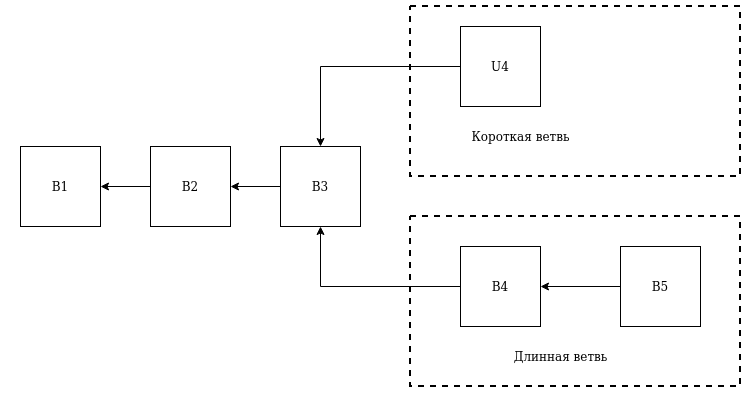
\includegraphics[width=\textwidth]{img/pow.png}
	\caption{Конкурирующие ветви блокчейна}
	\label{fig:a1}
\end{figure}

Генерация нового блока в PoW-консенсусе требует больших энергетических затрат, которые уходят впустую. Чтобы как-то компенсировать эти затраты некоторые проекты, как например \cite{primecoin}, осуществляют поиск простых чисел, что может пригодится в математических исследованиях.



\subsubsection{Алгоритм PoS}

Протокол PoS (англ. Proof of Stake -- <<подтверждение долей>>) является энергосберегающим аналогом PoW. Участники должны подтвердить факт владения некоторого количества валюты. Считается, что участники с б\'oльшим капиталом в сети будут меньше заинтересованы в атаке. Выбор валидаторов, основанный на их капитале в сети, не является абсолютно честным, поскольку единственный богатейший участник сможет контролировать консенсус всей сети. Поэтому решение о принятии нового блока принимается на основании комбинации размера доли и некоторого значения. Так, в проекте Blackcoin \cite{blackcoin} используется генератор псевдослучайных чисел, чтобы выбрать следующий блок, а в проекте Peercoin \cite{peercoin} отдается предпочтение возрасту денежных средств участника -- обладатели более старых сбережений имеют больше шансов валидировать следующий блок.

В отличие от PoW PoS гораздо более эффективный и менее энергозатратный. Однако факт того, что энергетическая цена валидации одного блока условно равна нулю, подвергает опасности сеть в начале ее существования. Поэтому многие проекты стартуют, используя PoW, а затем переходят к PoS. Например, Ethereum \cite{evm} планирует переход от Ethash (разновидность PoW) к Casper (разновидность PoS).



\subsubsection{Алгоритм DPoS}

Основное отличие DPoS (англ. Delegated PoS -- <<делегированный PoS>>) от PoS заключается в том, что PoS является непосредственно демократичным, а DPoS -- представительно демократичным \cite{dpos}. Держатели долей выбирают своих представителей, которые будут непосредственно создавать и валидировать новые блоки. Таким образом, можно существенно уменьшить количество валидаторов в сети, что влечет за собой быстрое подтверждение транзакций. Делегаты могут изменять параметры сети: размер блока, время до принятия нового блока. Однако участники сети могут не беспокоится в бесчестности делегатов, поскольку последние могут быть легко смещены на очередном голосовании.

\subsubsection{Алгоритм PBFT}

Алгоритм PBFT (англ. Practical Byzantine Fault Tolerance -- <<Практическая византийская отказоустойчивость>>) -- алгоритм репликации данных, разработанный для решения <<византийских>> ошибок \cite{pbft}. Каждый новый блок в сети определяется в очередном раунде. В каждом раунде, опираясь, на определенные правила, выбирается <<основной>> узел, который ответственен за последовательность транзакций в блоке. Весь процесс валидации может быть разбит на три этапа: предподготовка, подготовка и фиксирование. Чтобы приступить к следующему этапу узлу необходимо получить голоса от двух третей всех остальных участников, что свидетельствует о следующем:
\begin{itemize}[leftmargin=1.6\parindent]
	\item[---] PBFT устойчив к вредоносным узлам, если их количество не превышает треть участников сети;
	\item[---] каждый узел системы должен быть известен остальным членам сети.
\end{itemize}

Аналогично PoS и DPoS, на основании PBFT выработан алгоритм dPBFT, в котором путем голосования отбираются узлы, которые могут принимать участия в раундах валидации блоков \cite{dpbft}.


\subsubsection{Алгоритм Tendermint}

В протоколе Tendermint новый блок, аналогично PBFT, валидируется в очередном раунде \cite{tendermint}. Для начала выбирается узел-кандидат, чей блок планируется валидировать. Сам раунд валидации можно разделить на три этапа:
\begin{enumerate}[leftmargin=1.6\parindent]
	\item этап предголосования: участники решают, перейти ли к следующему этапу валидации блока;
	\item этап предфиксации: если на предыдущем этапе <<за>> проголосовало более двух третей участников, то в сеть транслируется информация об этом; если это подтверждает более двух третей узлов, то переходят к следующему этапу;
	\item этап фиксации: узел фиксирует факт валидации блока и транслирует эту информацию в сеть. Если он набирает более двух третей подтверждений, то сеть принимает этот блок.
\end{enumerate}

В отличие от PBFT, участники сети должны <<заморозить>> некоторую сумму на своих счетах, чтобы стать участником валидации.


\subsection{Сравнительный анализ рассмотренных средств и алгоритмов}

\subsubsection{Средства разработки блокчейн-сети}

Использование специализированной виртуальной машины (ВМ) позволяет порождать самые безопасные и ожидаемые результаты, но в то же время является самый ограниченным по возможным средствам разработки выбором. Нативный код, напротив, требует дополнительной проверки безопасности исполняемого кода, но зато почти неограничен в средствах разработки. Стандартна ВМ предоставляет компромисс между данными подходами. Отметим, что использование специализированной и стандартизированной ВМ позволяет вести учет затраченных ресурсов (чтобы, например, посчитать размер комиссии с валидации блока). В таблице 1 приведено сравнение виртуальных машин.

\begin{table}[h!]
	\captionsetup{justification=raggedleft,singlelinecheck=off}
	\caption{Сравнение вирутальных машин}
	\resizebox{\columnwidth}{!}{\begin{tabular}{| c | c  | c | c |}
			\hline
			\textbf{Характеристика} & \textbf{Спец. ВМ} & \textbf{Стандарт. ВМ} & \textbf{Нативный код} \\
			\hline
			Безопасность & $+$ & $+-$ & $-$ \\
			\hline
			Неограниченность средств & $-$ & $+-$ & $+$ \\
			\hline
			Учет затраченных ресурсов & $+$ & $+$ & $-$ \\
			\hline
	\end{tabular}}
\end{table}


Использование смарт-контрактов -- самая гибкая схема, поскольку позволяет проектировать произвольной сложности системы контрактов, однако требует более сложного устройства ВМ: требует от ВМ учет вычислительных ресурсов, проверку безопасности. Использование же нативного кода несколько усложняет проектирование систем контрактов, но зато предоставляют почти неограниченный функционал разработчикам. За проверку безопасности исполняемого нативного кода отвечают не ВМ, а валидаторы сети. В таблице 2 приведено сравнение способов обновления кода контрактов.

\begin{table}[h!]
	\captionsetup{justification=raggedleft,singlelinecheck=off}
	\caption{Сравнение способов обновления кода контрактов}
	\resizebox{\columnwidth}{!}{\begin{tabular}{|c | c  | c |}
			\hline
			\textbf{Характеристика} & \textbf{Смарт-контракты} & \textbf{Нативный код} \\
			\hline
			Безопасность & $-$ & $-$ \\
			\hline
			Неограниченность средств & $-$ & $+$ \\
			\hline
			Гибкость & $+$ & $-$ \\
			\hline
	\end{tabular}}
\end{table}


\subsubsection{Алгоритмы консенсуса}

Рассмотренные алгоритмы консенсуса имеет как свои преимущества, так и свои недостатки. В таблице 3 приведено сравнение алгоритмов консенсуса по следующим характеристикам:
\begin{enumerate}[leftmargin=1.6\parindent]
	\item[---] идентификация узлов: PBFT и Tendemint требуют идентификации каждого участника сети, чтобы выбрать очередного валидатора; в PoW, PoS и DPoS узлы могут свободно подключаться к сети;
	\item[---] энергоэффективность: в PoW для валидации блока необходимо выполнить внушительный объем вычислений, который уйдет впустую; PoS и DPoS также подбирают хэш блока, но поскольку они спроектированы так, чтобы свести поиск к минимуму, они экономят значительное число ресурсов; в Tendermint и PBFT отсутствует подбор хэша, что существенно экономит энергию;
	\item[---] допустимое число атакующих: в общем случае 51\% хэшируемой мощности сети является порогом для захвата всей сети, однако стратегия PoW позволяет снизить этот порог до 25\%; PBFT и Tendermint спроектированы выдерживать до трети атакующих от всего числа узлов; 
\end{enumerate}

\begin{table}[h!]
	\captionsetup{justification=raggedleft,singlelinecheck=off}
	\caption{Сравнение алгоритмов консенсуса}
	\resizebox{\columnwidth}{!}{\begin{tabular}{| p{5cm} | p{3cm}  | p{3cm} | p{3cm} | p{3cm} | p{3cm} |}
			\hline
			\textbf{Характеристика} & \textbf{PoW} & \textbf{PoS} & \textbf{DPoS} & \textbf{PBFT} & \textbf{Tendermint} \\
			\hline
			Идентификация узлов & нет & нет & нет & да & да \\
			\hline
			Энергоэффективность & нет & частичная & частичная & да & да \\
			\hline
			Допустимое число атакующих & <25\% вычислительной мощности & <51\% доли & <51\% валидаторов & <33.3\% византийских узлов & <33.3\% византийских голосующих \\
			\hline
	\end{tabular}}
\end{table}

PBFT и Tendermint -- протоколы, основанные на разрешениях. Идентификация узла сети должна доступна каждому участнику сети, таким образом, эти протоколы находят свое применение в корпоративных и приватных сетях. PoW, PoS и DPoS подходят для публичных сетей.


\subsection{Невзаимозаменяемые токены}

Невзаимозаменяемые токены (англ. Non-Fungible Tokens, NFTs) -- это тип криптовалюты, производной от Ethereum смарт-контрактов \cite{nft}. Если в классической криптовалюте денежная единица  является эквивалента другой единице и неотличима от нее, то NFT, напротив, является уникальным и не может быть обменен на себе подобный (буквально, невзаимозаменяемый) \cite{nft-pdf}. Данное свойство NFT позволяет его использовать для идентификации кого-то или чего-то в сети. Так, применение NFT позволяет доказать факт владения некоторым цифровым ресурсом, например, изображением, аудио- или видеозаписи, билетов на мероприятие и т.п.

Технология невзаимозаменямых токенов реализуется в блокчейн-сетях, которые гарантируют что информация о выдаче токена останется в истории сети, а проверка факта владения будет доступна любому частнику. Логика токена (его невзаимозаменяемость, прочие детали) прописывается в его смарт-контракте.


\subsection{Формализация предлагаемого метода}

Основываясь на проведенном анализе предметной области, задача по реализации метода создания уникальных сертификатов, подтверждающих окончание учебного заведения, с помощью технологии невзаимозаменяемых токенов может быть сформулирована следующим образом: необходимо спроектировать блокчейн-сеть на основе протокола консенсуса PBFT с использованием специализированной ВМ и смарт-контрактами для выдачи невзаимозаменяемых токенов. Входными данными являются документы об окончании учебного заведения, которые необходимо заверить невзаимозаменяемым токеном, а выходными данными -- блокчейн-сеть, содержащая невзаимозаменяемый токен. На основе сформулированной задачи была построена диаграмма IDEF0, представленная на рисунке \ref{fig:a2}.

\begin{figure}[!ht]
	\centering
	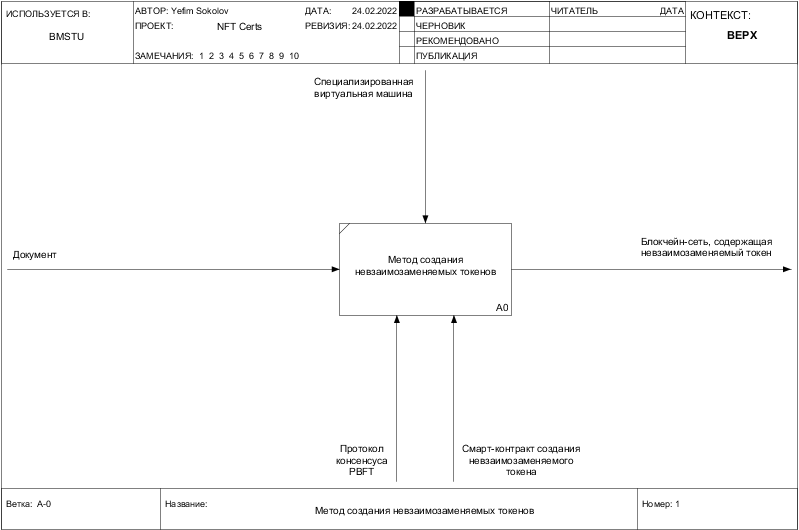
\includegraphics[width=\textwidth]{img/idef0_base.png}
	\caption{Концептуальная модель системы в нотации IDEF0}
	\label{fig:a2}
\end{figure}



\subsection*{Выводы}
\addcontentsline{toc}{subsection}{Выводы}
В аналитическом разделе был проведен анализ предметной области, включающий в себя обзор существующих методов выдачи сертификатов, подтверждающих окончание учебного заведения, а также средства разработки блокчейн-сети и алгоритм консенсунса сети. В ходе анализа была сформулирована задача разработки метода, проанализированы существующие методы решения поставленной задачи и предложен вариант её решения.


\pagebreak